\documentclass{article}
\usepackage[utf8]{inputenc}
\usepackage{amsmath}
\usepackage{amsfonts}
\usepackage{graphicx}
\usepackage{caption}
\usepackage{csquotes}
\usepackage{hyperref}


\title{An elliptic curve puzzle}
\author{Dave Neary}
\date{June 2021}

\begin{document}

\maketitle

\section{The origin story}

\begin{figure}[htb]
	\center{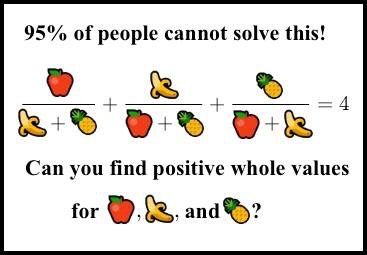
\includegraphics[width=0.4 \linewidth]{95_percent_cant_solve.jpeg}}
        \caption{"95\% of people cannot solve this!" is a low estimate}
	\label{fig:puzzle}
\end{figure}

Sometime in 2016, someone on the Math internet got annoyed with the silly and simple fruit problems on
Facebook, and made the puzzle in figure \ref{fig:puzzle}. It was intended as a cruel joke, because for
number theorists who tackled the problem, they recognized that this was a very difficult question
related to elliptic curves.

Rewriting the puzzle with normal mathematical symbols, the question asks you to find positive integer
solutions to the Diophantine equation:
\[ \frac{a}{b+c} + \frac{b}{c+a} + \frac{c}{a+b} = 4 \]

When you start to look at this puzzle, it becomes very quickly apparent that there is no easy answer to be
found. Frequent Quora contributor Alon Amit wrote
\href{https://www.quora.com/How-do-you-find-the-positive-integer-solutions-to-frac-x-y+z-+-frac-y-z+x-+-frac-z-x+y-4/answer/Alon-Amit}{a detailed account}
of the steps required to solve this puzzle, and showed that the smallest positive integer solution is:
\begin{equation*}
	\begin{split}
		a = &1544768021087461664419513150199198374856643256695654317000\\ &26634898253202035277999 \\
		b = &3687513179412999982719781156522547482549297996897197099628\\ &3137471637224634055579 \\
		c = &4373612677928697257861252602371390152816537558161613618621\\ &437993378423467772036
	\end{split}
\end{equation*}

Yes, those are 80-digit numbers.

Alon's article is a fascinating glimpse into a complex area of mathematics, and is peppered with comments like:
\begin{displayquote}
	When you find that your equation is an elliptic curve you A) rejoice and B) despair, because there’s
	so much to learn.
\end{displayquote}
\begin{displayquote}
	I know this looks like random voodoo, but please believe me that it’s not.
\end{displayquote}
\begin{displayquote}
	It’s the positive solutions that are the lair of dragons.
\end{displayquote}

At several points in his answer, I found myself wondering how to navigate the seemingly magic steps in his
solution. This is my attempt to explain in mind-numbing detail my voyage of discovery.

\section{Converting to Weierstrass normal form}

The first thing to do is to clear the denominators by multiplying across by $(a+b)(b+c)(c+a)$, at which point
we get to a cubic curve. By convention, when curves are in homogeneous form in 3 variables, we will use upper
case for variable names, for non-homogeneous curves in the affine plane we will use variable names in lower case.

\[ \mathcal{C}: A(A+B)(C+A) + B(B+C)(A+B) + C(C+A)(B+C) - 4(A+B)(B+C)(C+A) = 0 \]
\[ \mathcal{C}: A^3 + B^3 + C^3 -3(A^2B+B^2A+A^2C+C^2A+B^2C+C^2B) - 5ABC = 0 \]

This is a cubic curve, since each term in the expression is a monomial of degree 3. There are 3 variables,
$A, B, C$, but since each monomial has exactly degree 3, this is a homogeneous equation, and we can convert it
into a curve in two dimensions by dividing across by one of the variables. If we let
$a = \frac{A}{C}, b = \frac{B}{C}$ and divide across by $C^3$, we get:
\[ a^3 + b^3 -3a^2b -3 ab^2 -3a^2 -3b^2 -3a -3b -5ab +1 = 0 \]
which is a cubic curve in $\mathbb{R}^2$.

We will use the homogeneous form of the curve, however, along with some theory about the projective plane
$\mathbb{P}^2$. The projective plane is a superset of the regular 2d affine plane $\mathbb{A}^2$ which includes
"points at infinity", which are the intersection points of parallel lines of the same slope. It turns out to be
useful to generalize regular planar geometry to ensure that all distinct lines intersect in exactly one point.

We use $P = [X:Y:Z]$ to indicate points in the projective plane. Points in the plane are unique up to
multiplication by a scalar: the point $[tX:tY:tZ]$ is the same point as $[X:Y:Z]$. In this way, points in
$\mathbb{P}^2$ map directly to lines through the origin in $\mathbb{A}^3$, 3d affine space, and lines in
$\mathbb{P}^2$ map directly to planes through the origin in $\mathbb{A}^3$.

Our first challenge is to find a rational point on the curve $\mathcal{C}$. Since it is completely symmetrical in
$A, B, C$, by inspection we can take $[1:-1:0]$ (which we can easily check is on $\mathcal{C}$). Now we follow a
procedure to identify alternative axes for a linear transformation of $\mathbb{P}^2$ to transform the curve into a
curve into a new coordinate system $[X:Y:Z]$, and after setting $y = \frac{Y}{Z}, x=\frac{X}{Z}$, we end up with
an elliptic curve in Weierstrass normal form $y^2 = ax^3 + bx^2 + cx + d$. To be able to do this, we need a few things:
\begin{itemize}
	\item The $Z$ axis will be a tangent at infinity of $\mathbb{C}$
	\item The $Y$ axis will be a line of symmetry for the curve - $g(-Y,Z)=g(Y,Z)$
	\item Inspired by Alon Amit's answer, we will attempt to find an $X$ axis where the origin is a
		(rational) point on the transformed curve.
\end{itemize}

First up: let's find the tangent to our point $[1:-1:0]$ which will be our $Z$ axis. The tangent to a curve
$F(x,y,z)$ at the point $P=(a,b,c)$ is:
\[ \frac{\partial{F}}{\partial{x}}(P)(x-a) + \frac{\partial{F}}{\partial{y}}(P)(y-b) + 
\frac{\partial{F}}{\partial{z}}(P)(z-c) = 0 \]

For our curve $\mathcal{C}$:
\begin{equation*}
	\begin{split}
		\frac{\partial{F}}{\partial{A}} &= 3A^2 -6AB -3B^2 -6AC -3C^2 -5BC \\
		\frac{\partial{F}}{\partial{B}} &= 3B^2 -6AB -3A^2 -6BC -3C^2 -5AC \\
		\frac{\partial{F}}{\partial{C}} &= 3C^2 -6AC -3A^2 -6BC -3B^2 -5AB
	\end{split}
\end{equation*}

so the tangent at $[1:-1:0]$ is:
\[ 6(A-1) + 6(B+1) - C = 6A + 6B - C = 0 \]

Inspired by the symmetry in $A,B$, we will take our $Y$ axis to be $A - B = 0$.

Finally, for our $X$ axis, we will look for lines that intersect the affine version of our curve on the $X$ axis,
at a rational point. Setting $a=b$ in the affine curve above (since $A=B$ for the $Y$ axis, and
$a=\frac{A}{C}, b=\frac{B}{C}$) we get: 

\[ -4 a^3 -11a^2 -6a +1 = 0 \]

On inspection, we can see that $a=-1$ is a root, and we can factor it to give:
\[ -(a+1)(4a^2+7a-1) = 0 \]
\[ -(a + 1)(2a + \frac{1}{4}(7 + \sqrt{65}))(2a + \frac{1}{4}(7 - \sqrt{65})) = 0 \]

So we have our rational point at $a = b = -1$, which corresponds to a point in $\mathbb{P}^2 [-1:-1:1]$. Now we're
looking for a line parallel to $6A + 6B - C = 0$ which will be of the form $\alpha A + \alpha B + \gamma C = 0$ - 
setting $A=B=-1, C=1$, we see that $\gamma =2 \alpha$ and our $X$ axis is $ A + B + 2C = 0$.

Our transformation matrix is thus:
\[ 
\begin{pmatrix}
	1 & 1 & 2 \\
	1 & -1 & 0 \\
	6 & 6 & -1
\end{pmatrix}
\begin{pmatrix}
	A \\ B \\ C
\end{pmatrix}
 = 
\begin{pmatrix}
        X \\ Y \\ Z
\end{pmatrix}
\]

We can calculate the inverse of this matrix to generate the inverse linear transform to go from $(X,Y,Z)$ space
back to $(A,B,C)$ space too:
\[
	\frac{1}{26}
\begin{pmatrix}
        1 & 13 & 2 \\
        1 & -13 & 2 \\
        12 & 0 & -2
\end{pmatrix}
\begin{pmatrix}
        X \\ Y \\ Z
\end{pmatrix}
 =
\begin{pmatrix}
        A \\ B \\ C
\end{pmatrix}
\]

With this transform we can now change our curve from $(A,B,C)$ space to $(X, Y, Z)$ by setting:
\begin{equation*}
	\begin{split}
		A &= \frac{1}{26}\left(X + 13Y + 2Z\right) \\
		B &= \frac{1}{26}\left(X - 13Y + 2Z\right) \\
		C &= \frac{1}{26}\left(12X  - 2Z\right) \\
	\end{split}
\end{equation*}

After inserting these replacements into the equation of the curve $\mathcal{C}$ we get the following:
\begin{equation*}
	\begin{split}
		0 & =  \frac{1}{26^3}\left( (X+13Y+2Z)^3 + (X-13Y+2Z)^3 + (12X-2Z)^3  \right. \\
	          & - 3(X+13Y+2Z)^2(X-13Y+2Z) - 3(X+13Y+2Z)(X-13Y+2Z)^2 \\
		  & - 3(X+13Y+2Z)^2(12X-2Z) - 3(X-13Y+2Z)(12X-2Z)^2 \\
	          & - 3(X-13Y+2Z)^2(12X-2Z) - 3(X+13Y+2Z)(12X-2Z)^2 \\
	          & \left. - 5(X+13Y+2Z)(X-13Y+2Z)(12X-2Z) \right)
	\end{split}
\end{equation*}

Multiplying across by $26^3$, expanding, grouping terms, and dividing by a common factor of $26$, this
simplifies considerably to:
\[ 169Y^2Z + 28X^3 - 109 X^2Z + 8XZ^2 = 0 \]

By setting $p=\frac{Y}{Z}, q=\frac{X}{Z}$, we can dehomogenize the equation to its equivalent form:
\[ 169p^2 = -28q^3 + 109q^2 -8q \]

All that remains is to multiply by an appropriate factor for one last substitution to clear the
coefficients of the leading terms. $169=13^2$, and $28=2^2\times7$. We will need to multiply by
a perfect square to ensure that the coefficient of $p^2$ is a perfect square after substitution,
and we will want the exponents of all of the primes to be multiples of 3 for the $q^3$ term.
Combining these requirements, we can multiply across by $2^4\times7^2$ to give:

\[ (364p)^2 = (-28 q)^3 + 109(-28q)^2 + 224(-28q) \]

Setting $y = 364p, x = -28q$, we finally obtain the Weierstrass form of the initial equation:
\[ y^2 = x^3 + 109x^2 +224x \]

And we can reverse the substitution steps to find values of $A, B, C$ that correspond to any point
$x,y$ on the resulting curve:

\begin{equation*}
	\begin{array}{lllll}
		y &= 364p & \quad \mathrel{\#} \text{Final substitution} \\
		 &= 364\frac{Y}{Z} & \quad \mathrel{\#} \text{Homogenization} \\
		 &= 364\frac{A - B}{6A + 6B - C} & \quad \mathrel{\#} \text{Transformation from $(X,Y,Z)$ to $(A,B,C)$} \\
		x &= -28q & \quad \mathrel{\#} \text{Final substitution} \\
		 &= -28\frac{X}{Z} & \quad \mathrel{\#} \text{Homogenization} \\
		 &= -28\frac{A + B +2C}{6A + 6B - C} & \quad \mathrel{\#} \text{Transformation from $(X,Y,Z)$ to $(A,B,C)$} \\
	\end{array}
\end{equation*}

And we can also do something similar to translate any point on the curve in $(A,B,C)$ space to a point in
$(X,Y,Z)$ space by considering $\frac{A}{A+B+C}, \frac{B}{A+B+C}, \frac{C}{A+B+C}$ (which works since
$[A:B:C] \in \mathbb{P}^2$ is a point in projective space):

\begin{equation*}
	\begin{array}{lllll}
		\frac{A}{A+B+C} &= \frac{\frac{1}{26}\left(X + 13Y + 2Z\right)} {\frac{1}{26}\left(14X+2Z\right)}
		& \quad \mathrel{\#} \text{Transformation from $(A,B,C)$ to $(X,Y,Z)$} \\
		 &= \frac{\frac{X}{Z} + 13\frac{Y}{Z} + 2}{14\frac{X}{Z}+2} & \quad \mathrel{\#} \text{Dehomogenization} \\
		 &= \frac{\frac{-x}{28} + \frac{y}{28} + 2}{\frac{-x}{2} + 2} & \quad \mathrel{\#} x=-28\frac{X}{Z}, y=364\frac{Y}{Z} \\
		 &= \frac{56 - x + y}{56 - 14x} & \quad \mathrel{\#} \text{Simplification} \\
		\frac{B}{A+B+C} &= \frac{\frac{1}{26}\left(X - 13Y + 2Z\right)} {\frac{1}{26}\left(14X+2Z\right)}
		& \quad \mathrel{\#} \text{Transformation from $(A,B,C)$ to $(X,Y,Z)$} \\
		 &= \frac{\frac{X}{Z} - 13\frac{Y}{Z} + 2}{14\frac{X}{Z}+2} & \quad \mathrel{\#} \text{Dehomogenization} \\
		 &= \frac{\frac{-x}{28} - \frac{y}{28} + 2}{\frac{-x}{2} + 2} & \quad \mathrel{\#} x=-28\frac{X}{Z}, y=364\frac{Y}{Z} \\
		 &= \frac{56 - x - y}{56 - 14x} & \quad \mathrel{\#} \text{Simplification} \\
		\frac{C}{A+B+C} &= \frac{\frac{1}{26}\left(12X - 2Z\right)} {\frac{1}{26}\left(14X+2Z\right)}
		& \quad \mathrel{\#} \text{Transformation from $(A,B,C)$ to $(X,Y,Z)$} \\
		 &= \frac{12\frac{X}{Z} - 2}{14\frac{X}{Z}+2} & \quad \mathrel{\#} \text{Dehomogenization} \\
		 &= \frac{\frac{-3x}{7} - 2}{\frac{-x}{2} + 2} & \quad \mathrel{\#} x=-28\frac{X}{Z} \\
		 &= \frac{-28 - 6x}{28 - 7x} & \quad \mathrel{\#} \text{Simplification} \\
	\end{array}
\end{equation*}


In summary: given any solution $(x,y)$ to our transformed equation, as long as a few conditions are met
(like $28-7x \neq 0$) we can find a solution in $[A:B:C]$ with:
\[ A = \frac{56 - x + y}{56 - 14x}, B = \frac{56 - x - y}{56 - 14x}, C = \frac{-28 - 6x}{28 - 7x} \]

And similarly, given $A, B, C$ solving our original equation, we  can generate $(x,y)$ which solve our transformed
equation with:
\[ x = -28\frac{A + B + 2C}{6A + 6B - C}, y = 364\frac{A - B}{6A + 6B - C} \]

\section{Group operations on elliptic curves}

We now get to the theory of elliptic curves which is kind of magic. In the projective plane, two curves of 
degree $n$ and $m$ are guaranteed to have $n\times m$ (potentially identical) intersection points. Given a
cubic curve $\mathcal{C}$ and a line $L: \alpha X + \beta Y + \gamma Z = 0$ through two points on the curve
$\mathcal{C}$, we are guaranteed to be able to find a third intersection point (potentially a point at
infinity).

Given this, and given that (by design) for our curve $\mathbb{C}$ we have $f(X,Y,Z) = f(X,-Y,Z)$, we can
define an addition operator for points on the curve as follows:

Given two points $P_1, P_2 \in \mathcal{C}$, the line $\alpha X + \beta Y + \gamma Z = 0$ through $P_1, P_2$
intersects $\mathcal{C}$ at a third point $P_1*P_2 = [X_3:Y_3:Z_3]$. We then use the symmetry of $\mathcal{C}$
in the X axis to define the point $P_3 = P_1 + P_2$ as $[X_3:-Y_3:Z_3]$. Using this operator, and with the zero
element $\mathcal{O}$ equal to the point at infinity ($[0:1:0]$ for $\mathcal{C}$), the points of the curve $C$
are a well defined group. This operation of "flipping" the $Y$ value of the point is equivalent to taking the
line through $\mathcal{O}$ and $P_1*P_2$ and finding the third intersection point. In other words:
\[ P_1 + P_2 = \mathcal{O}*(P_1*P_2) \]

We can also add a point to itself by taking a tangent to $\mathcal{C}$ at $P$.

To be a group, this operator has to satisfy a few conditions:
\begin{enumerate}
	\item $P + \mathcal{O} = P$ for all $P \in \mathcal{C}$.
	\item $P + Q = Q + P$ for all $P, Q \in \mathcal{C}$.
	\item $(P + Q) + R = P + (Q + R)$ for $P,Q,R \in \mathcal{C}$.
	\item For all $P \in \mathcal{C}$, there exists a point $-P \in \mathcal{C}$ such that $P+(-P) = \mathcal{O}$.
\end{enumerate}

We can verify that all of these conditions are met - and the points of the curve $\mathcal{C}$ form
a group under addition with this operator. What's more, we can identify a number of subgroups, in
particular, the set of rational points on the curve (that is,
$\{[X:Y:Z] \in \mathcal{C} : X,Y,Z \in \mathbb{Q}\}$) forms a group, since any line joining two rational
points has a rational slope, and is guaranteed to meet the curve at a rational point, since all of the
coefficients of the curve are integers.

\begin{figure}[htb]
        \center{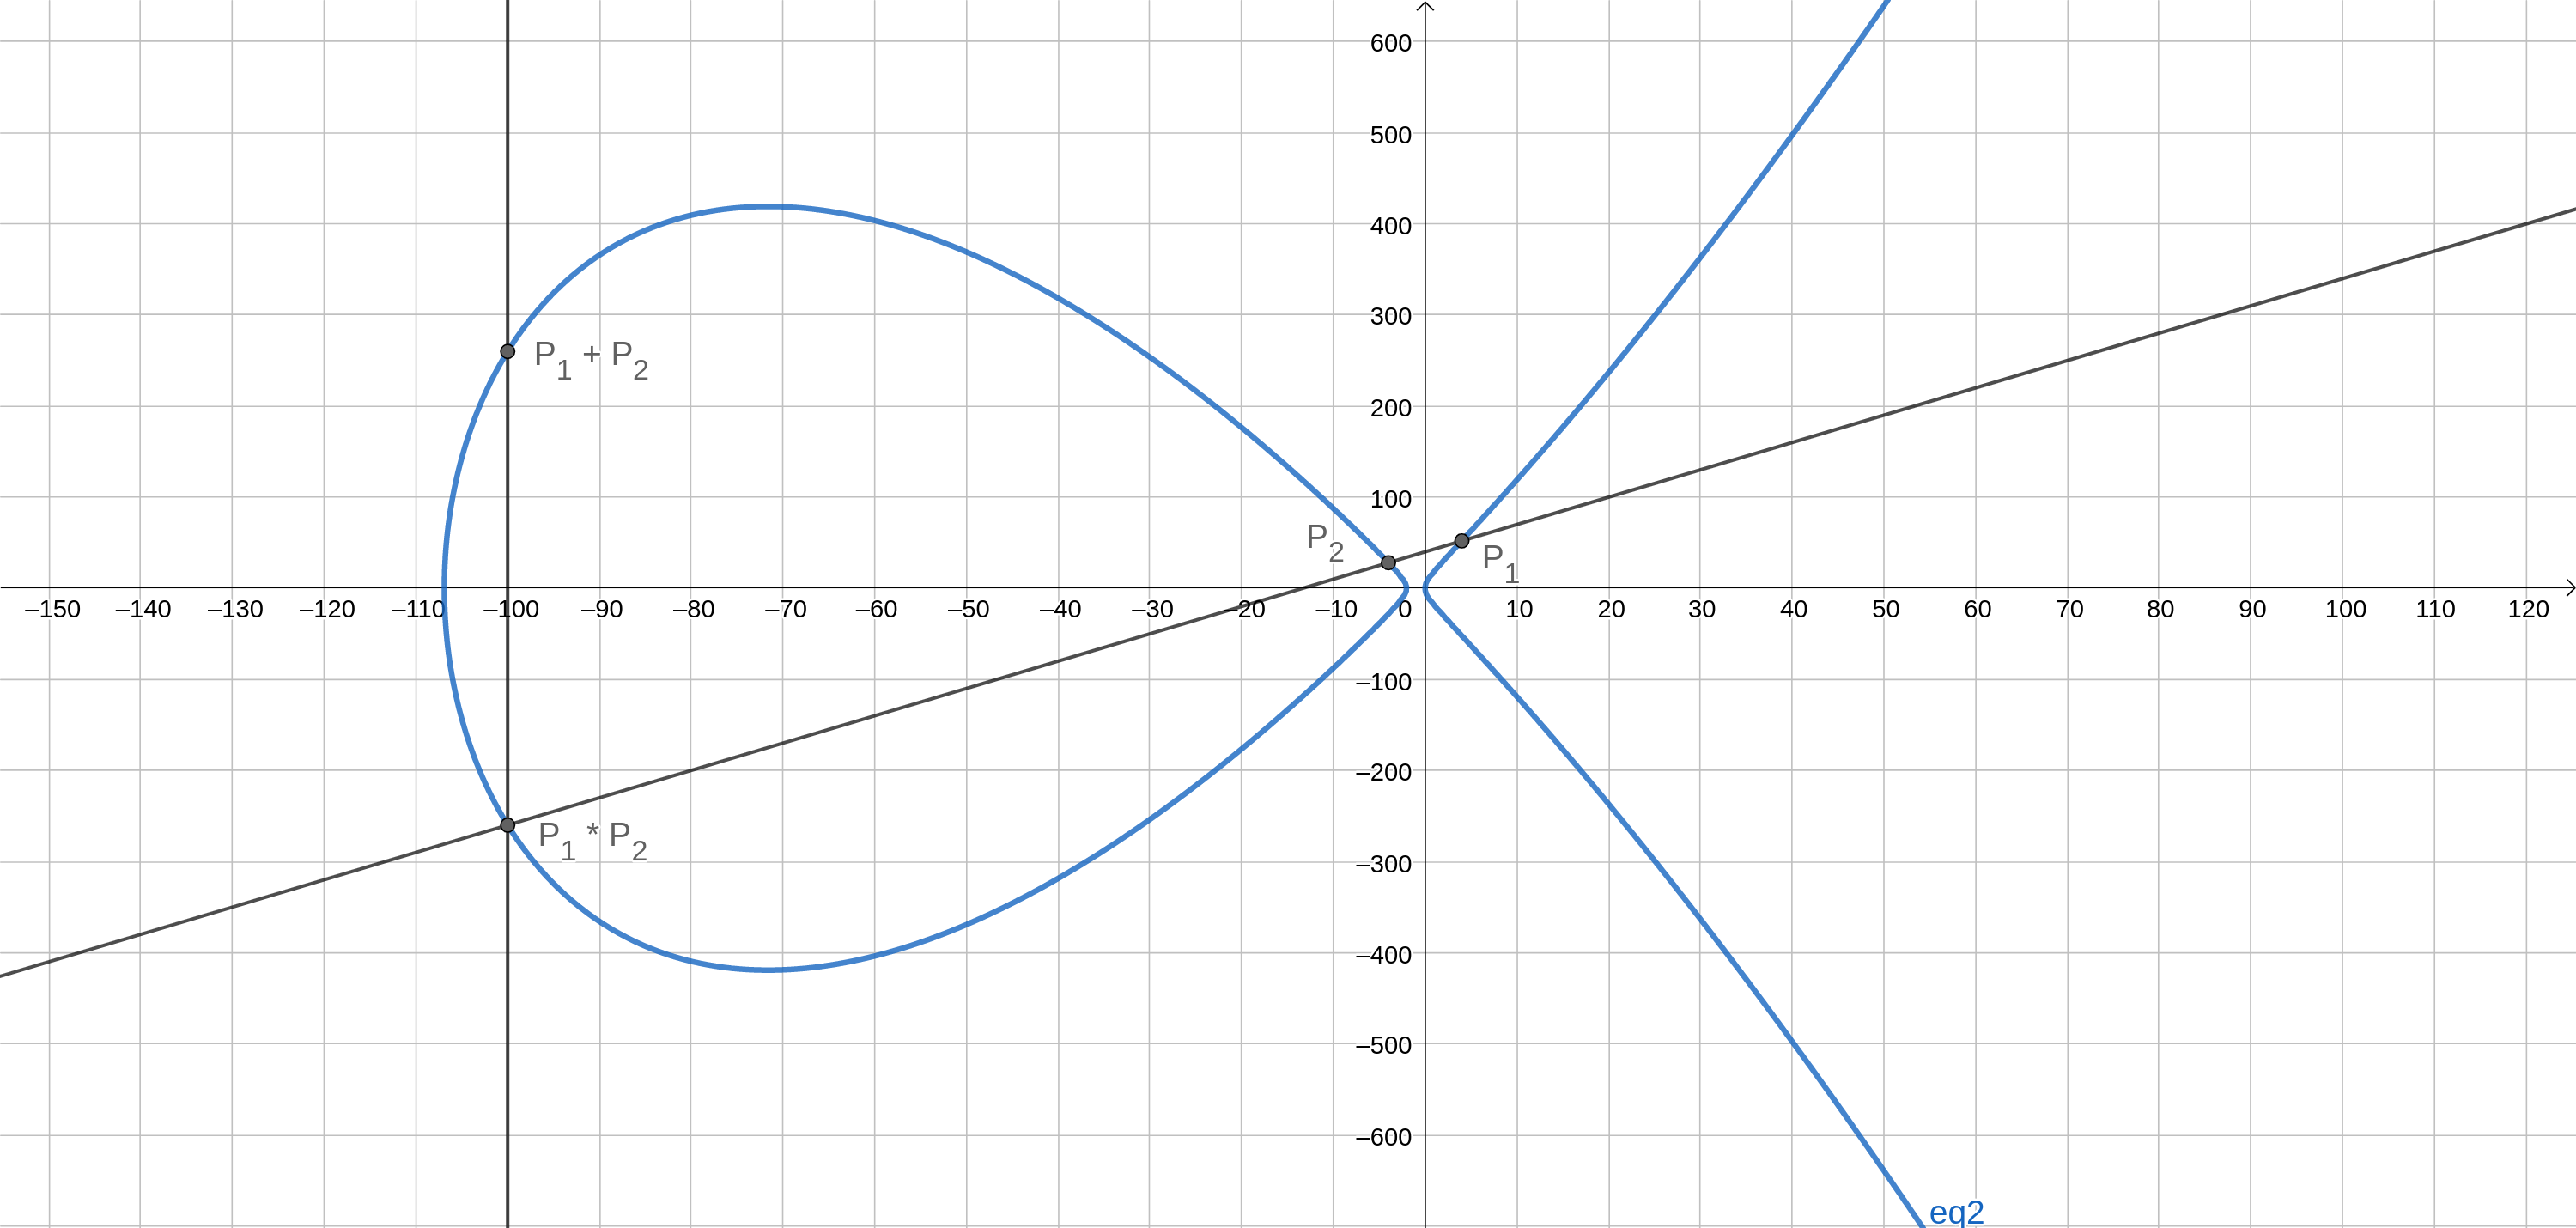
\includegraphics[width=0.9 \linewidth]{elliptic_curve_addition.png}}
	\caption{Addition of points on an elliptic curve}
	\label{fig:ecc_addition}
\end{figure}


We can also find subgroups of finite order. For a curve with three real roots, for example, we can show
that $2P = \mathcal{O}$ for the roots, so these points are of order 2. We can also find points of order
3 by finding the inflection points of the curve. There are several nice results that prove that these
points of finite order are guaranteed to be integers, and can have a limited number of orders related to
the determinant of the curve. But that's not helpful to us right now.

One interesting idea is that if we find a point of infinite order on the curve, all of the multiples of
that point also form a subgroup, and in fact, all rational points on the curve will be a member of one of
a finite number of subgroups generated from rational points.

\section{Finding rational points on $\mathcal{C}$}

We have already identified some rational points on the curve $\mathcal{C}$ in the projective space
$[X,Y,Z]$ - specifically, the point at infinity $\mathcal{O}: [0:1:0]$, and the origin $[0:0:1]$. This is
the only rational point of order 2 on $\mathcal{C}$.

We can also calculate the two other roots of $y^2=x^3+109x^2+224x$ using the quadratic equation, but
they are not rational:
\[ x = \frac{1}{2}(-109 \pm 13\sqrt{65}) \]

To find the points of order 3, we look for the inflection points of the curve. For the most part, we can stay
in the affine plane here. Using implicit differentiation, we calculate the 2nd derivative and set it equal to zero:
\begin{equation*}
	\begin{split}
		y^2 &= x^3 + 109x^2 + 224x \\
		2y\, \frac{dy}{dx} &= 3x^2 + 218x + 224 \\
		\frac{dy}{dx} &= \frac{3x^2+218x+224}{2y} \\
		\frac{d^2y}{dx^2} &= \frac{2y(6x+218) - (2\frac{dy}{dx})(3x^2+218x+224)}{4y^2} \\
		&= \frac{4y^2(6x+218) - 2(3x^2+218x+224)^2}{8y^3} \\
		&= \frac{4(x^3 + 109x^2 + 224x)(6x+218) - 2(3x^2+218x+224)^2}{8y^3} \\
		&= \frac{3x^4+436x^3+1344x^2-50176}{4y^3} 
	\end{split}
\end{equation*}

Setting the second derivative equal to zero, we discover that it has a root at $x=4$, giving another rational
point $(x,y) = (4,52)$. The slope of the tangent to $\mathcal{C}$ at that point is:
\[ \frac{dy}{dx} = \frac{3x^2+218x+224}{2y} = \frac{3(16) + 218(4) + 224}{104} = 11 \]
giving a tangent line of $y = 11x + 8$ which we can substitute back into the equation for the curve to
find the other intersection point (if one exists):
\begin{equation*}
	\begin{split} 
		(11x+8)^2 &= x^3+109x^2+224x \\
		121x^2+176x+64 &= x^3+109x^2+224x \\
		x^3-12x^2+48x-64 &= 0 \\
		(x-4)^3 &= 0
	\end{split}
\end{equation*}

So the points at $x=4$ are triple roots, and given $P=(4,52)$, $2P = (4,-52)$, and $3P = \mathcal{O}$.

This is not particularly helpful in finding solutions to our original equation, however, because these
values of $(x,y)$ do not work in our rational relation since $x=4$ results in a division by zero. To
find the desired positive integer solutions, we will need to find a rational point of infinite order.
Unfortunately, there is no guaranteed way to do this (in fact, there are curves which have no rational
points of infinite order), but we do have some techniques we can try.

The first, unsatisfactory in general because the smallest solution to the equation can be very large, or
be a rational number with a very large denominator, is trial and error. In the case of this curve, it is
not too hard to find the points $(x,y) = (-4,\pm28)$. Once we have found one such point, we can find many
others using our addition operator. Given $P_1 = (4,52), P_2=(-4,28)$, we can find the equation of the
line through these points:
\begin{equation*}
	\begin{split}
		y - y_1 &= \frac{y_2 - y_1}{x_2 - x_1} (x - x_1) \\
		y - 52 &= \frac{52 - 28}{4 - (-4)} (x - 4) \\
		y &= 3x + 40
	\end{split}
\end{equation*}

Substituting this back into the curve, and using the fact that we have (by design) intersection points at
$x=\pm 4$, we get:
\begin{equation*}
        \begin{split}
		x^3 + 109x^2 + 224x &= (3x + 40)^2 \\
                 &= 9x^2 + 240x + 1600 \\
		 x^3 +100 x^2 - 16x - 1600 &= 0 \\
		 (x - 4)(x + 4) (x + 100) &= 0
        \end{split}
\end{equation*}

Plugging in $x = -100$ into the line equation, we get $y = -260$, so $P_1 * P_2 = (-100, -260)$ and
$P_1 + P_2 = (-100, 260)$. The point $(x,y) = (-4,28)$ maps to 
$(A, B, C) = (\frac{11}{14}, \frac{4}{14}, \frac{-1}{14})$ in our original equation, and multiplying across 
by 14 to clear denominators, we find that:
\begin{equation*}
	\begin{split}
		\frac{11}{4 - 1} + \frac{4}{11 - 1} + \frac{-1}{11+4} &= \frac{11}{3} + \frac{2}{5} - \frac{1}{15} \\
		&= \frac{55 + 6 - 1}{15} = 4
	\end{split}
\end{equation*}

The point $(-100, 260)$ maps to $\left(\frac{2}{7},\frac{-1}{14}, \frac{11}{14}\right)$, giving the same solution again.

Given the seed point $P = (-4,28)$ we can now start calculating other points using our doubling rule.
The tangent line at $(-4,28)$ is:
\[ y - 28 = \frac{3(-4)^2+218(-4)+224}{2(28)}(x+4) \]
\[ 7y = -75x - 104 \]

Substituting this, and using our double root at $x=-4$, we find:
\begin{equation*}
        \begin{split}
		49(x^3 + 109x^2 + 224x) &= (-75x -104)^2 \\
                 49x^3 + 5341 x^2 + 10976 x &= 5625x^2 + 15600x + 10816 \\
                 49x^3 - 284 x^2 - 4624 x - 10816 &= 0 \\
                 (x - 4)^2 (49x - 676) &= 0
        \end{split}
\end{equation*}

Giving us a new point $2P = (\frac{676}{49},\frac{55796}{343})$, which maps to $(A,B,C) = 
(\frac{-366}{245}, \frac{1033}{1176}, \frac{1357}{840})$ - which, after clearing denominators, gives the integer
solution: $(A,B,C) = (-8784, 5165, 9499)$.

The tangent at $2P$ is the hairy looking equation:
\[ y = \frac{1141223}{97643}x + \frac{525512}{368039} \]

which intersects the curve twice at $x=\frac{676}{49}$ and once more at:
\[ x = \frac{102131236}{9534155449} \] 
(yes, I used a computer to calculate this!) giving:
\[ 4P = (\frac{102131236}{9534155449}, -\frac{1445821255910884}{930943540506707})\].

\[ (A,B,C) = (6334630576523495, 6696085890501216, -6531563383962071) \]

which are already becoming ridiculously big numbers.

Now if we double down again and calculate $8P$, we end up with the tangent line:
\begin{equation*}
	\begin{split}
		336494489729383006652049074747 y &= \\
		 -24519383769572153108112248149367 x &- 259944632223927427391370958376 
	\end{split}
\end{equation*}

After substitution, this has a double root at $4P$ and one more root at:
\[ x = \frac{6478053524552625623839628465124452884145956}{1245636875525200464539184202153614229609} \] 
\[ y = - \frac{16659913412846099183252330384510918009297731314186105439712688964}{43962986240372060709927105816763012422999312489817805553227} \]

giving $8P = (x,-y)$.

As we generate further multiples of our seed point $P$, the solutions are getting more and more complicated.
We can continue to find new points by finding new multiples of $P$, ideally aided by a computer. Eventually,
we will find $9P$, which is the first multiple to give a positive integer solution to the original problem,
the 80 digit numbers in the first section.

But what if, for a different value of $N$ than 4, the smallest solution was not so easy to find by
experiment? What other methods are there to find a rational point we can use to generate an infinite group?


\end{document}

